\documentclass{beamer}

\mode<presentation> { \usetheme{Madrid} }
\usepackage{amsmath, amsthm, amssymb, amsfonts,listings,graphicx,caption,subcaption,hyperref,mathtools, multicol, booktabs, scrextend}
%----------------------------------------
%	TITLE PAGE
%----------------------------------------

\title[DS8004 Project Presentation I]{DS8004 Project Presentation 1:\\ Twitter topic classification}
\author{Anil Trikha, Pengshuai Shi}
\institute[Ryerson]
{
Ryerson University \\
\medskip
}
\date{\today}

\begin{document}

\begin{frame}
\titlepage
\end{frame}

\begin{frame}
\frametitle{Overview}
\tableofcontents
\end{frame}

%-----------------------------------------------------
%	PRESENTATION SLIDES
%-----------------------------------------------------
\section{Problem} 
\begin{frame}
%\fontsize{6pt}{12}\selectfont
\frametitle{Introduction and problem}
\begin{itemize}
\item People use the hashtag symbol (\#) before a relevant keyword or phrase in their Tweet to categorize those Tweets and help them show more easily in Twitter search.
\item Hashtagged words that become very popular are often Trending Topics.\cite{twitter_sup} 
\end{itemize}
\begin{figure}[h]
	\centering
	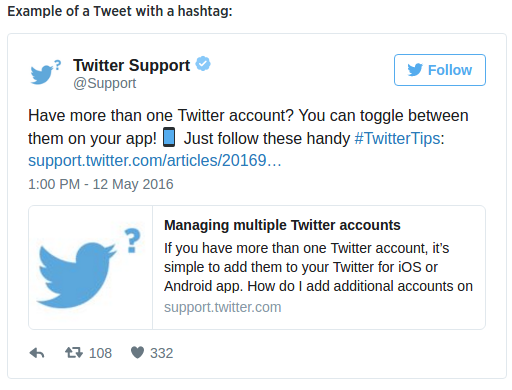
\includegraphics[width=0.3\textwidth]{twitter_hashtag.png}
\end{figure}
Only 14.6\% of tweets contain hashtags, a reliable hashtag classification system could help researchers to label the rest of tweets. And existing machine learning models are mostly conventional and reaches a bottleneck because they are using TF-IDF which ignores the semantic information.\cite{paper}  
\end{frame}
%------------------------------------------------
\section{Proposed solution}
\begin{frame}
\frametitle{Proposed solution}
Recurrent neural networks (RNNs) have recently achieved promising results in many ML tasks, and inspired by the recent improvement of document level sentiment classification, a LSTM-RNN model is proposed to learn semantic tweet representations. \cite{paper}
\begin{figure}[h]
%\centering
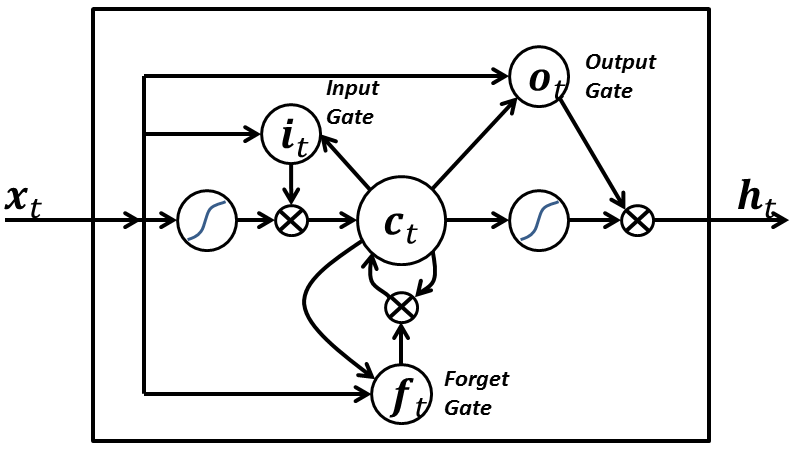
\includegraphics[width=0.5\textwidth]{lstm.png}
\cite{lstm} \textit{Wiki}
\end{figure}
\end{frame}
%------------------------------------------------
\section{Methodology}
\begin{frame}
\frametitle{Steps}
\begin{enumerate}
\item Obtain tweets using Twitter REST/Search API 
\item Data preprocessing, e.g. tokenization, word representation
\item Utilize CNN to compose sentence representations
\item Use LSTM to encode the intrinsic relations between words
\item Compare result with conventional methods such as SVM
\end{enumerate}
\end{frame}

%------------------------------------------------
\section{Schedule}
\begin{frame}
\frametitle{Schedule}
1. Researching on how LSTM is implemented.\\
2. Choose which tool to use.\\
3. Try to reproduce some basic result in the paper \cite{paper}.\\
\end{frame}
%------------------------------------------------
\section{Expected outcomes}
\begin{frame}
\frametitle{Expected outcomes}
1. Be able to produce topic label when we feed in a tweet.\\
2. Obtain similar result as stated in the paper. \\
3. Produce the most trending topic during the time of the project.\\
\end{frame}
%------------------------------------------------
\begin{frame}
\frametitle{References}
\begin{thebibliography}{9}
	\bibitem{twitter_sup} 
	Twitter hashtag
	\\\texttt{https://support.twitter.com/articles/49309}
	\bibitem{paper}
	Jia Li, Hua Xu, Xingwei He, Junhui Deng and Xiaomin Sun, 
	\textit{Tweet modeling with LSTM recurrent neural networks for hashtag recommendation}, 2016
	\bibitem{lstm}
	Long short-term memory\\
	\text{https://en.wikipedia.org/wiki/Long\_short-term\_memory}
\end{thebibliography}
\end{frame}

%----------------------------------------------------------------------------------------

\end{document}